\chapter{MINE/SEEKS/MANTA} 
\label{sec:ships}
\lstset{style=6502Style}

Every few frames, a decision is required: should we launch a \textit{Uridimine} at the player,
potentially thoroughly ruining their day? Life and death matters are best left to computers,
or the gods. Since we have a computer, and it has a source of random numbers available
, we can resolve this dilemma between god and machine by choosing
a bit of both:  we can read in a a byte of white noise from the \icode{\$D41B} register, random
static generated by the Commodore 64's sound chip. This will tell us what to do, whether to kill
or go in peace.

\begin{minipage}[c]{0.30\linewidth}
	\vspace{-0.1cm}
	\begin{figure}[H]
		\centering
		\begin{adjustbox}{width=4.0cm,center}
			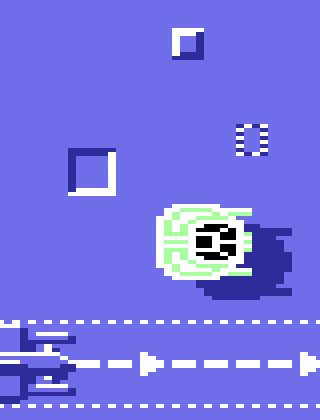
\includegraphics{src/uridimine/level9_MaybeLaunchUridimine.png}%
		\end{adjustbox}
	\end{figure}
\end{minipage}
\begin{minipage}[c]{0.68\linewidth}
\begin{lstlisting}[basicstyle=\scriptsize\ttfamily]
MaybeLaunchUridimine
  LDA uridimineInProgress  ; Is one in progress already?
  BPL DontLaunchUridimine  ; If so, skip.
  LDA fireBulletOrMine     ; Does the level allow one?
  BEQ DontLaunchUridimine  ; If not, skip.
  LSR                      ; Divide by 2.
  LSR                      ; Divide by 2 again.
  CMP $D41B                ; Compare to random number.
  BCC DontLaunchUridimine  ; Skip if less.
  LDX uridimineArrayIndex  ; Get index to available sites. 
  BMI DontLaunchUridimine  ; If none, skip.
FindSuitableSite   
  LDA uridimineLaunchSiteXPosArray,X ; Get candidate site.
  BPL LaunchUridimine      ; If available, launch!
  DEX                      ; Check the next site.
  BPL FindSuitableSite     ; Keep looping until no more.
DontLaunchUridimine   
  RTS
\end{lstlisting}
\end{minipage}

There are many trapdoors on the way to this life or death decision. We may have already
launch a mine, the level may not allow one, but the final determination is whether
the value we've tuned for the level (\icode{fireBulletOrMine}) is less then some random
number. If it is: the player lives to fight on. Otherwise, it is possibly curtains for
their ambitions of completing the level.

Once we've decided to launch a mine though, and found a suitable launch site we call
\fcode{LaunchUridimine} to get the job done.

\begin{minipage}[c]{0.30\linewidth}
	\vspace{-0.1cm}
	\begin{figure}[H]
		\centering
		\begin{adjustbox}{width=4.0cm,center}
			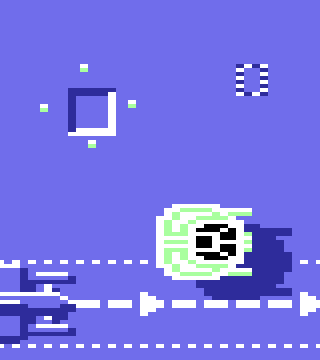
\includegraphics{src/uridimine/level9_LaunchUridimine.png}%
		\end{adjustbox}
	\end{figure}
\end{minipage}
\begin{minipage}[c]{0.68\linewidth}
\begin{lstlisting}[basicstyle=\scriptsize\ttfamily]
LaunchUridimine
  LDA #$FF               ; Put -1 in A and..
  STA spriteEnable       ; ..use it to enable sprite.
  LDA #$1D               ; Load the initial sprite value. 
  STA currentSpriteValue ; And store it.
  LDA #$08               ; AnimateMineCreation is now..
  STA indexToEnemyUpdatePtrArray,Y ; ..active.
  LDA uridimineLaunchSiteYPosArray,X ; Get site Y pos.
  STA currentSpriteYPos  ; Position the sprite with it.
  LDA uridimineLaunchSiteXPosArray,X ; Get site X pos.
  STA currentSpriteXPos  ; Position the sprite with it.

  JSR DisplayCurrentSprite ; Display the sprite.
  INC uridimineInProgress; Flag uridimine in progress.
  RTS
\end{lstlisting}
\end{minipage}

\begin{wrapfigure}[3]{l}{0.9cm} % <==========================================
    \vspace{-0.4cm}
    \begin{adjustbox}{width=1.2cm,left}
      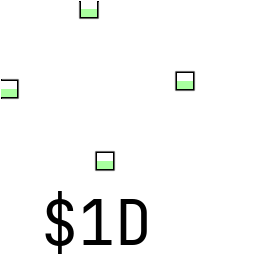
\includegraphics{src/uridimine/level9_launch_1D.png}%
    \end{adjustbox}
\end{wrapfigure}
When a uridimine launch is performed, it does not immediately pop into existence. There is a flourish,
or more concretely, a launch sequence.
\icode{S1D} is set as the initial sprite for this sequence. Thanks to the X and Y positions
stored in \fcode{uridimineLaunchSiteXPosArray} and \fcode{uridimineLaunchSiteYPosArray}
it can be placed directly over the launch silo. The uridimine is born like a star, from a sort of 
implosion, in which its constituent parts appear to materialize and then coalesce:

\begin{figure}[H]
  \centering
  \begin{adjustbox}{width=13.0cm,center}
    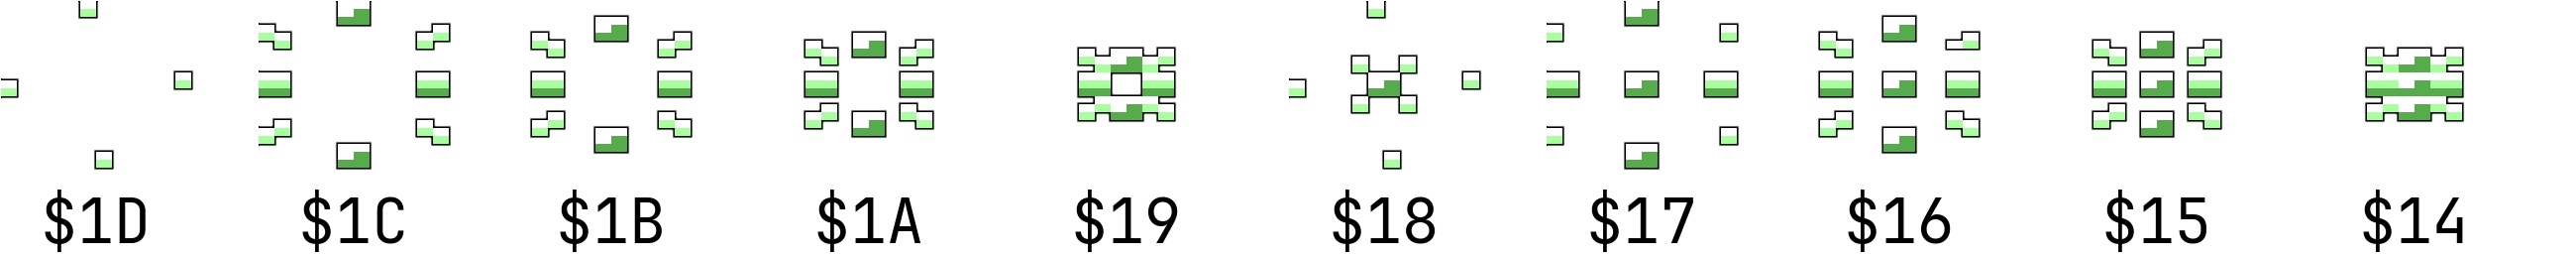
\includegraphics{src/uridimine/level9_launch_sequence.png}%
  \end{adjustbox}
\end{figure}
\vspace{-0.4cm}

This process of creation is managed by the \fcode{AnimateMineCreation} routine, a chunk of code
just as compact as its predecessor. 

\begin{minipage}[c]{0.30\linewidth}
	\vspace{-0.1cm}
	\begin{figure}[H]
		\centering
		\begin{adjustbox}{width=4.0cm,center}
			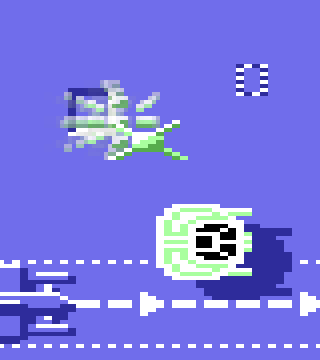
\includegraphics{src/uridimine/level9_launch.png}%
		\end{adjustbox}
	\end{figure}
\end{minipage}
\begin{minipage}[c]{0.68\linewidth}
\begin{lstlisting}[basicstyle=\scriptsize\ttfamily]
AnimateMineCreation
  JSR FollowMantaOnX    ; Move towards the manta.
  LDA frameRate         ; Check the frame rate.
  AND #$03              ; Make it between 0 and 7.
  BNE SkipAnimating     ; Don't update unless 0.
  DEC currentSprite     ; Move to next sprite.
  LDA currentSprite     ; Check progress..
  CMP #$14              ; If it's reached $14 then..
  BCS SkipAnimating     ; .. we're finished launching.
  LDA #$0A              ; Set function to MineSeeksManta
  STA indexToEnemyUpdatePtrArray,Y
  LDA #$11              ; Set sprite to uridimine.
  STA currentSprite     ; Store it.
SkipAnimating   
  JMP DetectLeavingScreen  ; Check if left the screen.
\end{lstlisting}
\end{minipage}

\begin{wrapfigure}[3]{l}{0.9cm} % <==========================================
    \vspace{-0.2cm}
    \begin{adjustbox}{width=1.4cm,left}
      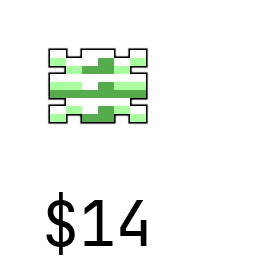
\includegraphics{src/uridimine/level9_launch_14.png}%
    \end{adjustbox}
\end{wrapfigure}
This routine is called every frame or two, and cycles the sprite through each
phase of the sequence until it reaches \icode{\$14}, the last stage. While doing this it even manages to take
time to start moving the nascent uridimine in the direction of the player. Even though it isn't yet fully formed,
the uridimine is already a menace - beginning its implacable, lethal journey. 

\begin{wrapfigure}[3]{l}{0.9cm} % <==========================================
    \vspace{-0.6cm}
    \begin{adjustbox}{width=1.4cm,left}
      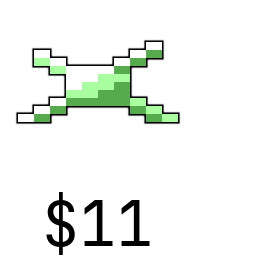
\includegraphics{src/uridimine/level9_launch_11.png}%
    \end{adjustbox}
\end{wrapfigure}
Once the implosion of creation is complete
it installs the final incarnation of the uridimine (sprite \icode{\$11}) in position. The uridimine is now fully active
and control is now passed to \fcode{MineSeeksManta}, which will shepherd it towards the player no matter where they 
run or hide.

As we would expect, \fcode{MineSeeksManta} is preoccupied completely with homing in on the player and figuring out
whether we have hit them yet. Most of this work is delegated out to the routine \fcode{UpdateMineVelocity}, which does
the difficult (and complex) part of working out how to adjust the uridimine's speed and direction to improve its chances
of detonating next to the manta. It also has to check if the uridimine has run out of time yet - the allotted time
for the mine is stored in \fcode{movementDuration}. Once it has run out it is time to call \fcode{MineExpired} and
put this failed uridimine to bed.

\begin{minipage}[c]{0.30\linewidth}
	\vspace{0.0cm}
	\begin{figure}[H]
		\centering
		\begin{adjustbox}{width=4.0cm,center}
			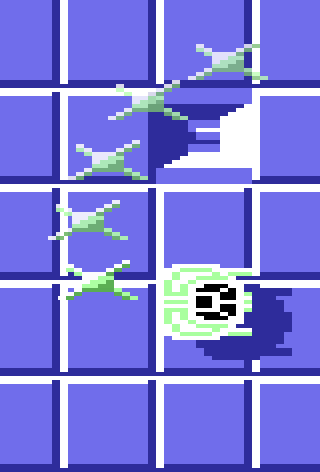
\includegraphics{src/uridimine/level9_seek.png}%
		\end{adjustbox}
	\end{figure}
\end{minipage}
\begin{minipage}[c]{0.68\linewidth}
\begin{lstlisting}[basicstyle=\scriptsize\ttfamily]
MineSeeksManta
  JSR FollowMantaOnX         ; Follow Manta along X axis.
  JSR UpdateEnemySpriteXYPos ; Update new position.
  JSR UpdateMineVelocity     ; Follow Manta along Y axis. 
  LDA movementDuration,Y     ; Update duration..
  SBC #$01                   ; .. by subtracting 1.
  STA movementDuration,Y     ; If we've reached zero..
  BEQ MineExpired            ; .. the mine has expired.

  JSR DetectHittingManta     ; Have we hit the manta?
  BCC DetectLeavingScreen    ; No, check if left screen.
  INC hasMantaBeenHit        ; Yes, flag manta as hit.
  JMP DetectLeavingScreen    ; Done for now.

MineExpired
  LDA #$14                   ; Set sprite to 'explode'
  STA currentSpriteValue     ; Store it.
  LDA #$06                   ; AnimateUridimineExplosion
  STA indexToEnemyUpdatePtrArray,Y
  JMP DetectLeavingScreen    ; Done for now.
\end{lstlisting}
\end{minipage}

\begin{wrapfigure}[3]{l}{0.9cm} % <==========================================
    \vspace{-0.6cm}
    \begin{adjustbox}{width=1.4cm,left}
      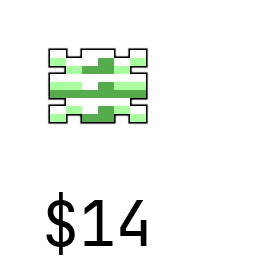
\includegraphics{src/uridimine/level9_launch_14.png}%
    \end{adjustbox}
\end{wrapfigure}
An expired uridimine ends where it began. We replace the active sprite with \icode{\$14} - marking the 
beginning of its explosive finale. This sequence is the exact reverse of the one that gave birth to it.
To manage this sequence we hand control to the final routine responsible for managing the uridimine, 
\fcode{AnimateUridimineExplosion}.

\begin{figure}[H]
  \centering
  \begin{adjustbox}{width=13.0cm,center}
    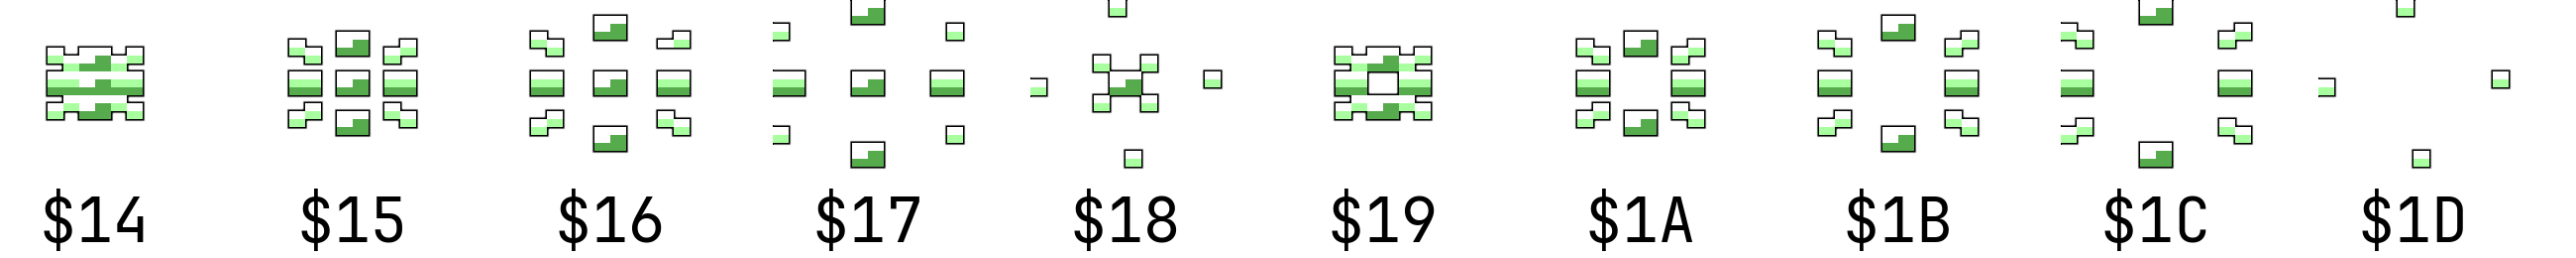
\includegraphics{src/uridimine/level9_uridimine_explodes_sequence.png}%
  \end{adjustbox}
\end{figure}

This routine doesn't have much to do other than run the animation to completion. Notice that
even in death, the uridimine will continue to follow the manta, oblivious to its own fate.
We can also note that the \fcode{frameRate} of the explosion is higher (and the resulting
animation faster) than the one that managed its birth. Here we will animate a new frame
of the explosion at every second opportunity, while the birth of the uridimine animated
every 7th frame. In the illustration below, where we superimpose each frame of the explosion
on top of the other, we notice something pleasing. Each frame is circumscribed by the same eight-spoked
star shape. 

\begin{minipage}[c]{0.30\linewidth}
	\vspace{-0.1cm}
	\begin{figure}[H]
		\centering
		\begin{adjustbox}{width=4.0cm,center}
			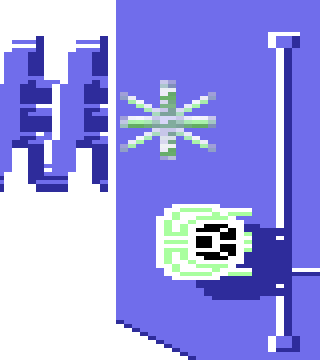
\includegraphics{src/uridimine/level9_explodes.png}%
		\end{adjustbox}
	\end{figure}
\end{minipage}
\begin{minipage}[c]{0.68\linewidth}
\begin{lstlisting}[basicstyle=\scriptsize\ttfamily]
AnimateUridimineExplosion
  JSR FollowMantaOnX      ; Follow Manta along X axis.
  LDA frameRate           ; Check the frame rate.
  AND #$01                ; Make it between 0 and 1.
  BNE DetectLeavingScreen 
  INC currentSpriteValue  ; Move to next sprite.
  LDA currentSpriteValue  ; Check progress..
  CMP #$1E                ; If it's reached $1E then..
  BCC DetectLeavingScreen ; .. we're finished launching.
  LDA #$00                ; Put $00 in A.
  STA spriteEnable        ; Disable the sprite.
  LDY currentEnemyIndex   ; Get the mine's index.
  STA indexToEnemyUpdatePtrArray,Y ; Store 0 in function.
  DEC uridimineInProgress  ; Free up a slot.
  JSR DisplayCurrentSprite ; Display erased sprite.
  RTS
\end{lstlisting}
\end{minipage}

One last thing worth noting is the way this entire control sequence was orchestrated. Throughout we've
passed control of the uridimine from one routine to another, by updating the active function in 
\fcode{indexToEnemyUpdatePtrArray}. In the \fcode{UpdateEnemies} routine opposite we see how the contents
of this array are used to figure out which routine to call for each active enemy, including the uridimine.


\clearpage
\begin{lstlisting}[basicstyle=\scriptsize\ttfamily]
UpdateEnemies
        LDA #$0A
        STA dataIndex
        LSR
        ; Store $08 in currentEnemyIndex
        STA currentEnemyIndex
        LDA #$FF
        STA currentSpriteMultiColorMode
        STA spriteEnable
        LDA #$00
        STA currentSpriteBackgroundDisplayPriority

EnemyUpdateLoop   
        LDY currentEnemyIndex
        STY spriteIndex
        LDA indexToEnemyUpdatePtrArray,Y
        AND #$0E
        BEQ SkipEnemyUpdate

        ; Run a function for the sprite.
        TAX
        LDA enemyUpdatePtrArray,X
        STA functionHiPtr
        LDA enemyUpdatePtrArray + $01,X
        STA functionLoPtr

        JSR GetCurrentSprite
        LDY currentEnemyIndex
functionHiPtr   =*+$01
functionLoPtr   =*+$02
        JSR UpdateEnemyPositions

SkipEnemyUpdate
        DEC dataIndex
        DEC dataIndex
        DEC currentEnemyIndex
        BPL EnemyUpdateLoop
        RTS
\end{lstlisting}
